\chapter{Method}


\section{Image texture analysis methods}
\subsection{Co-occurrence matrix}


The co-occurence matrix (COM) is second-order statistics methods, which is based on information about gray levels in pair of pixes. The matrix is defined over the image with distribution values at a given offset. Mathematically we have a COM matrix \textbf{C} which is defined over an $n \times m$ image \textbf{I}, with $\Delta x, \Delta y$ being the parameterized offset, is calculated by

\[
C_{\Delta x, \Delta y}(i, j) = \Sigma_{p=1}^n\Sigma_{q=1}^m
\begin{dcases}
  1, \quad \text{if } I(p,q)=i \text{ and } I(p+\Delta x, q+ \Delta y) =j \\
  0, \quad \text{otherwise}
\end{dcases}
\]
\fxnote[inline]{find reference}

The element (5,4) in the COM can be translated to meaning how many times there exist an element in the image with GI \fxnote[inline]{level or intensity?} 5 and another element offset $\Delta x, \Delta y$ from the originial with greyscale intensity  (GI) 4, i.e. if the offset is (,1) and the first element is (x,y)(4,3) with GI 5 it would mean that element (x,y)(5,3) would have GI 4. If COM(4,4) is ten, it translates into there being ten instances with element (x,y) = 5 and (x+$\Delta x$,y+$\Delta y$) = 4.

\begin{figure}[H]
  \centering
  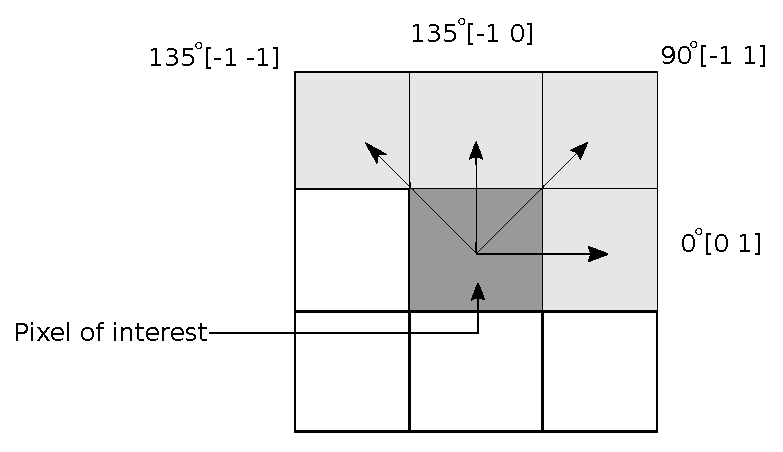
\includegraphics[scale=0.5]{2DCOM.eps}
  \caption{Example of the offsets for the 2D}\label{2DCOM}
\end{figure}

\begin{figure}[H]
  \centering
  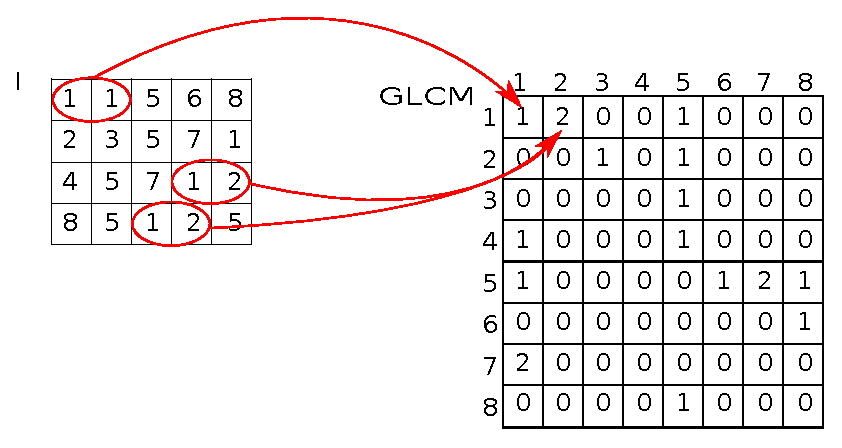
\includegraphics[scale=0.8]{GLCM.eps}
  \caption{Example how the values in the GLCM are calclulated of the 4-by-5 image I. Element (1, 1) in the GLCM contains the value 1 because there is only one instance inf the image where two horizontally adjacent pixels have the values 1 and 1.}\label{GLCM}
\end{figure}


A single image have multiple COMs as different offsets creates different relations. Consider a 3 $\times$ 3 matrix looking at element (2,2) we can then create eight different offsets, {(1,0),(1,1), (0,1)),(-1,1),(-1,0),(-1,-1),(0,-1),(1,-1)}, however they are not unique. \fxnote[inline]{Lave 3x3 matrice med offsets.}

Focusing on the two offsets {(0,1), (0,-1)} in element (2,2) and (1,2) with GI 1 and 2 respectfully increases the entry COMs$_{1,0}$(1,2) and COMs$_{-1,0}$ (1,1) with one, showing that COMs$_{0,1}$$^\textbf{T}$ = COMs$_{0,-1}$. There exist the same relation between (1,1)(-1,-1), (0,1)(0,-1), and (-1,1)(1,-1). This leaves four different offsets for analysis {(0,1),(-1,1), (-1,0)),(-1,-1)} in general {(0,d),(-d,d),(-d,0),(-d,-d)} where d is the distance which are commonly named angles 0$^\circ$, 45$^\circ$, 90$^\circ$ and 135$^\circ$.
\fxnote[inline]{show 3x3 matrix with angles clearly visible}\\

The co-occurrence matrix is quadratic with the number of rows and columns equal to the amount of GI, for example if we have 256 GI we get a 256 $\times$ 256 COM.
\fxnote[inline]{Show example on a 5x5 matrix with GI 8, offset [1 0] and [0 1]}\\

Extending this method to three-dimensions it is necessary to look on how the offsets are defined because the size of the COM is defined by the amount of GIs and not by the images it is derived from. Considering a 3 $\times$ 3 $\times$ 3 matrix we have a possible of 26 offsets. In two-dimensions it is possible to eliminate half of the offsets because of the relation COM$_{d,d}^\textbf{T}$ = COM$_{-d,-d}$, and it is the same case in three-dimensions with the relation being COM$_{d,d,d}^\textbf{T}$ = COM$_{-d,-d,-d}$. This leaves 13 offsets which are illustrated below.\\
\fxnote[inline]{3 gange 3 gange, farv de ønskede dele eller noget}

\begin{figure}[H]
  \centering
  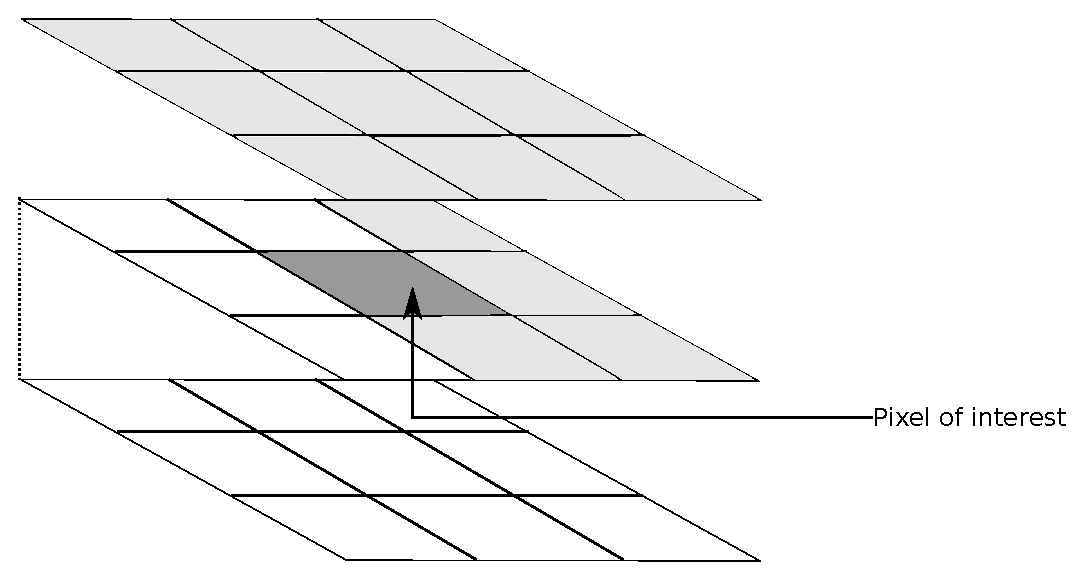
\includegraphics[scale=0.8]{3DCOM.eps}
  \caption{Example of the offsets for the 3D}\label{3DCOM}
\end{figure}


\subsection{Texture features from co-occurrence matrix}

\section{Machine learning methods}

\subsection{Crossval}



\subsection{Feature selection}

\subsubsection{Naive}

\subsubsection{Sequential Forward Feature}

\subsection{K-nearest neighbors algorithm}

k-NN for short is a method that is used for classification and regression. Where the output is a class and member of this class, and this object is classified by its neighbors. For instance, if we chose k to 1, then the object will be assigned to the class of the single nearest neighbor.

The algorithm consist of training examples, that are vectors in multidimensional space, with each its label. The most used distance metric is Euclidean distance.

The drawback of k-NN is that classification can be skewed in that way, that the more frequent class tend to dominate the prediction of new examples, because they tend to be common among the k-NN due to their large number.

The way we wish to implement the k-NN in matlab is, first we handle the data, then we will calculate the distance between two data instances and after that, we can locate k most similar data instances and generate a response from a set. After all this is done, we have to summarize the accuracy of predictions.


Dette vil være en lille introduktion til de tools vi bruger til at analysere vores data med. Da vores data er MRI skanninger af hjernen, som er nogen voxels\footnote{noget her} som bliver repræsenteret i 3D.\\



\section{Erode}
Normalt brugte man dette til binære billeder, men senere hen er det udvidet til også at omfatte grayscale billeder. Grunden til at dette bruges er for at fjerne støj på billedet.

Vi bruger Erode på vores MRI scanning, da der kan være gray-bit mix og derfor fjerner overflydig og blandet data. Hvis vi starter på hvordan 2D virker, så

For at illustrere hvordan erosion virker, gør vi det på et 2D plan, betragt figur \ref{Erosion2D}, hvor vi bruger et plus til at fjerne støj.
\begin{figure}[H]
  \centering
    \begin{tikzpicture}[scale=0.5]
    \matrix[square matrix]
    {
    |[fill=white]| & |[fill=white]|   & |[fill=white]|   & |[fill=white]|   & |[fill=white]|\\
    |[fill=white]| & |[fill=white]|   & |[fill=red!30]|$N_2$ & |[fill=white]|   & |[fill=white]|\\
    |[fill=white]| & |[fill=red!30]|$N_1$ & |[fill=red!30]|$\boxplus$ & |[fill=red!30]|$N_3$ & |[fill=white]|\\
    |[fill=white]| & |[fill=white]|   & |[fill=red!30]|$N_4$ & |[fill=white]|   & |[fill=white]|\\
    |[fill=white]| & |[fill=white]|   & |[fill=white]|   & |[fill=white]|   & |[fill=white]| \\
    };
    \end{tikzpicture}
  \caption{Text}\label{Erosion2D}
\end{figure}
Så med figur \ref{Erosion2D}, bruger vi denne på figur \ref{ErosionExample}.
\begin{figure}[H]
  \centering
    \begin{tikzpicture}
    \matrix[square matrixlarge]
    {
    |[fill=white]| & |[fill=white]| & |[fill=white]| & |[fill=white]| & |[fill=white]| & |[fill=white]| & |[fill=white]| & |[fill=white]| & |[fill=white]| & |[fill=white]| \\
    |[fill=white]| & |[fill=white]| & |[fill=white]| & |[fill=white]| & |[fill=white]| & |[fill=white]| & |[fill=white]| & |[fill=white]| & |[fill=white]| & |[fill=white]| \\
    |[fill=white]| & |[fill=white]| & |[fill=white]| & |[fill=blue!30]| & |[fill=blue!30]| & |[fill=white]| & |[fill=white]| & |[fill=white]| & |[fill=white]| & |[fill=white]| \\
    |[fill=white]| & |[fill=white]| & |[fill=blue!30]| & |[fill=blue!30]| & |[fill=blue!30]| & |[fill=blue!30]| & |[fill=white]| & |[fill=white]| & |[fill=white]| & |[fill=white]| \\
    |[fill=white]| & |[fill=white]| & |[fill=blue!30]| & |[fill=blue!30]| & |[fill=blue!30]| & |[fill=blue!30]| & |[fill=white]| & |[fill=white]| & |[fill=white]| & |[fill=white]| \\
    |[fill=white]| & |[fill=white]| & |[fill=white]| & |[fill=blue!30]| & |[fill=blue!30]| & |[fill=blue!30]| & |[fill=blue!30]| & |[fill=white]| & |[fill=white]| & |[fill=white]| \\
    |[fill=white]| & |[fill=white]| & |[fill=white]| & |[fill=blue!30]| & |[fill=blue!30]| & |[fill=blue!30]| & |[fill=blue!30]| & |[fill=white]| & |[fill=white]| & |[fill=white]| \\
    |[fill=white]| & |[fill=white]| & |[fill=white]| & |[fill=white]| & |[fill=white]| & |[fill=blue!30]| & |[fill=white]| & |[fill=white]| & |[fill=white]| & |[fill=white]| \\
    |[fill=white]| & |[fill=white]| & |[fill=white]| & |[fill=white]| & |[fill=white]| & |[fill=white]| & |[fill=white]| & |[fill=white]| & |[fill=white]| & |[fill=white]| \\
    |[fill=white]| & |[fill=white]| & |[fill=white]| & |[fill=white]| & |[fill=white]| & |[fill=white]| & |[fill=white]| & |[fill=white]| & |[fill=white]| & |[fill=white]| \\
    };
    \end{tikzpicture}
    \begin{tikzpicture}
    \matrix[square matrixlarge]
    {
    |[fill=white]| & |[fill=white]| & |[fill=white]| & |[fill=white]| & |[fill=white]| & |[fill=white]| & |[fill=white]| & |[fill=white]| & |[fill=white]| & |[fill=white]| \\
    |[fill=white]| & |[fill=white]| & |[fill=white]| & |[fill=white]| & |[fill=white]| & |[fill=white]| & |[fill=white]| & |[fill=white]| & |[fill=white]| & |[fill=white]| \\
    |[fill=white]| & |[fill=white]| & |[fill=white]| & |[fill=red!50]| & |[fill=red!50]| & |[fill=white]| & |[fill=white]| & |[fill=white]| & |[fill=white]| & |[fill=white]| \\
    |[fill=white]| & |[fill=white]| & |[fill=red!50]| & |[fill=blue!30]| & |[fill=blue!30]| & |[fill=red!50]| & |[fill=white]| & |[fill=white]| & |[fill=white]| & |[fill=white]| \\
    |[fill=white]| & |[fill=white]| & |[fill=red!50]| & |[fill=blue!30]| & |[fill=blue!30]| & |[fill=red!50]| & |[fill=white]| & |[fill=white]| & |[fill=white]| & |[fill=white]| \\
    |[fill=white]| & |[fill=white]| & |[fill=white]| & |[fill=red!50]| & |[fill=blue!30]| & |[fill=blue!30]| & |[fill=red!50]| & |[fill=white]| & |[fill=white]| & |[fill=white]| \\
    |[fill=white]| & |[fill=white]| & |[fill=white]| & |[fill=red!50]| & |[fill=red!50]| & |[fill=blue!30]| & |[fill=red!50]| & |[fill=white]| & |[fill=white]| & |[fill=white]| \\
    |[fill=white]| & |[fill=white]| & |[fill=white]| & |[fill=white]| & |[fill=white]| & |[fill=red!50]| & |[fill=white]| & |[fill=white]| & |[fill=white]| & |[fill=white]| \\
    |[fill=white]| & |[fill=white]| & |[fill=white]| & |[fill=white]| & |[fill=white]| & |[fill=white]| & |[fill=white]| & |[fill=white]| & |[fill=white]| & |[fill=white]| \\
    |[fill=white]| & |[fill=white]| & |[fill=white]| & |[fill=white]| & |[fill=white]| & |[fill=white]| & |[fill=white]| & |[fill=white]| & |[fill=white]| & |[fill=white]| \\
    };
    \end{tikzpicture}
    \begin{tikzpicture}
    \matrix[square matrixlarge]
    {
    |[fill=white]| & |[fill=white]| & |[fill=white]| & |[fill=white]| & |[fill=white]| & |[fill=white]| & |[fill=white]| & |[fill=white]| & |[fill=white]| & |[fill=white]| \\
    |[fill=white]| & |[fill=white]| & |[fill=white]| & |[fill=white]| & |[fill=white]| & |[fill=white]| & |[fill=white]| & |[fill=white]| & |[fill=white]| & |[fill=white]| \\
    |[fill=white]| & |[fill=white]| & |[fill=white]| & |[fill=white]| & |[fill=white]| & |[fill=white]| & |[fill=white]| & |[fill=white]| & |[fill=white]| & |[fill=white]| \\
    |[fill=white]| & |[fill=white]| & |[fill=white]| & |[fill=blue!30]| & |[fill=blue!30]| & |[fill=white]| & |[fill=white]| & |[fill=white]| & |[fill=white]| & |[fill=white]| \\
    |[fill=white]| & |[fill=white]| & |[fill=white]| & |[fill=blue!30]| & |[fill=blue!30]| & |[fill=white]| & |[fill=white]| & |[fill=white]| & |[fill=white]| & |[fill=white]| \\
    |[fill=white]| & |[fill=white]| & |[fill=white]| & |[fill=white]| & |[fill=blue!30]| & |[fill=blue!30]| & |[fill=white]| & |[fill=white]| & |[fill=white]| & |[fill=white]| \\
    |[fill=white]| & |[fill=white]| & |[fill=white]| & |[fill=white]| & |[fill=white]| & |[fill=blue!30]| & |[fill=white]| & |[fill=white]| & |[fill=white]| & |[fill=white]| \\
    |[fill=white]| & |[fill=white]| & |[fill=white]| & |[fill=white]| & |[fill=white]| & |[fill=white]| & |[fill=white]| & |[fill=white]| & |[fill=white]| & |[fill=white]| \\
    |[fill=white]| & |[fill=white]| & |[fill=white]| & |[fill=white]| & |[fill=white]| & |[fill=white]| & |[fill=white]| & |[fill=white]| & |[fill=white]| & |[fill=white]| \\
    |[fill=white]| & |[fill=white]| & |[fill=white]| & |[fill=white]| & |[fill=white]| & |[fill=white]| & |[fill=white]| & |[fill=white]| & |[fill=white]| & |[fill=white]| \\
    };
    \end{tikzpicture}
  \caption{Left: Middle: Right:}\label{ErosionExample}
\end{figure}
Således er støjen nu fjernet. Vi vil udvide dette til 3D, da vores MRI er i 3D. Som det ses på figur \ref{Erosion2D} har denne 4 naboer den tjekker, når man udvider til 3D, får vi 2 nye naboer, dvs 6 naboer i alt. Hvis en af dem er udenfor den ønskede matrix, eksluderes pixlen.


Da vores data er i 3D, så i udvider vi erosion, hvor det stadig er et plus, men med 2 ekstra naboer
Now we expand this cross for the 3D and its the same concept for 3D. Now it 6 neighbours instead of 4, where we expand it for the 3D
\begin{figure}[H]
  \centering
    \begin{tikzpicture}
    \matrix[square matrix]
    {
    |[fill=white]| & |[fill=white]|   & |[fill=white]|   & |[fill=white]|   & |[fill=white]|\\
    |[fill=white]| & |[fill=white]|   & |[fill=white]| & |[fill=white]|   & |[fill=white]|\\
    |[fill=white]| & |[fill=white]| & |[fill=red!30]|$N_5$ & |[fill=white]| & |[fill=white]|\\
    |[fill=white]| & |[fill=white]|   & |[fill=white]| & |[fill=white]|   & |[fill=white]|\\
    |[fill=white]| & |[fill=white]|   & |[fill=white]|   & |[fill=white]|   & |[fill=white]| \\
    };
    \end{tikzpicture}
    \begin{tikzpicture}
    \matrix[square matrix]
    {
    |[fill=white]| & |[fill=white]|   & |[fill=white]|   & |[fill=white]|   & |[fill=white]|\\
    |[fill=white]| & |[fill=white]|   & |[fill=red!30]|$N_2$ & |[fill=white]|   & |[fill=white]|\\
    |[fill=white]| & |[fill=red!30]|$N_1$ & |[fill=red!30]|$\boxplus$ & |[fill=red!30]|$N_3$ & |[fill=white]|\\
    |[fill=white]| & |[fill=white]|   & |[fill=red!30]|$N_4$ & |[fill=white]|   & |[fill=white]|\\
    |[fill=white]| & |[fill=white]|   & |[fill=white]|   & |[fill=white]|   & |[fill=white]| \\
    };
    \end{tikzpicture}
    \begin{tikzpicture}
    \matrix[square matrix]
    {
    |[fill=white]| & |[fill=white]|   & |[fill=white]|   & |[fill=white]|   & |[fill=white]|\\
    |[fill=white]| & |[fill=white]|   & |[fill=white]| & |[fill=white]|   & |[fill=white]|\\
    |[fill=white]| & |[fill=white]| & |[fill=red!30]|$N_6$ & |[fill=white]| & |[fill=white]|\\
    |[fill=white]| & |[fill=white]|   & |[fill=white]| & |[fill=white]|   & |[fill=white]|\\
    |[fill=white]| & |[fill=white]|   & |[fill=white]|   & |[fill=white]|   & |[fill=white]| \\
    };
    \end{tikzpicture}
  \caption{Text}\label{Erosion3D}
\end{figure}



\fxnote[inline]{Vi billede af eroded og original mask}



Image texture
PCA
Principal Component Analysis Application to images
Machine learning (Knn, Ann, Gaussian)


\small
noget tekst \fxfatal{her er noget galt}

noget mere tekst \fxnote[inline]{en note}

endnu mere tekst \fxwarning{en advarsel -- noget er helt forkert}

og til slut mere tekst \fxerror[inline]{en fejl}
